% Generated by paper/build_imt_mixing_figure.py; do not hand edit.
% Q1 producer SHA-256: 1c65c5da992e7b646fdfb09d33bd1874dc344281122d2ba7bf6d9a46103cbf1a
\begin{figure}[tb]
\centering
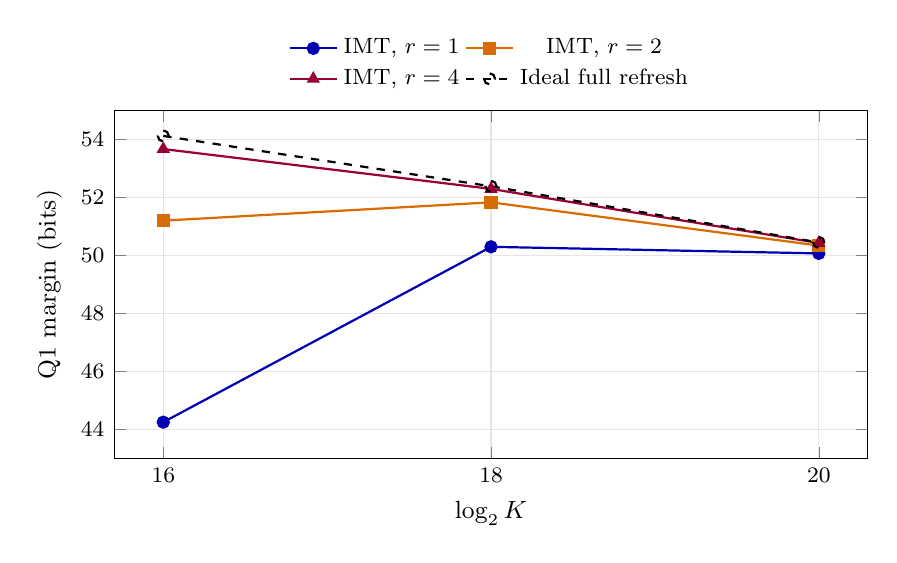
\begin{tikzpicture}
\begin{axis}[width=.92\linewidth,height=6cm,
tick label style={font=\footnotesize},label style={font=\small},
grid=major,grid style={black!10},
xlabel={$\log_2 K$},ylabel={Q1 margin (bits)},
xmin=15.7,xmax=20.3,ymin=43,ymax=55,xtick={16,18,20},ytick={44,46,48,50,52,54},
legend style={font=\footnotesize,draw=none,at={(.5,1.03)},anchor=south,legend columns=2}]
\addplot[blue!70!black,thick,mark=*] coordinates {(16,44.2557080902) (18,50.3041855097) (20,50.0765838679)};
\addlegendentry{IMT, $r=1$}
\addplot[orange!85!black,thick,mark=square*] coordinates {(16,51.2066374038) (18,51.8381868608) (20,50.3473485316)};
\addlegendentry{IMT, $r=2$}
\addplot[purple!80!black,thick,mark=triangle*] coordinates {(16,53.6773528963) (18,52.3019654202) (20,50.4353872190)};
\addlegendentry{IMT, $r=4$}
\addplot[black,dashed,thick,mark=o] coordinates {(16,54.1283826857) (18,52.3901851833) (20,50.4554997999)};
\addlegendentry{Ideal full refresh}
\end{axis}
\end{tikzpicture}
\caption{Effect of mixing depth $r$ on the length curve, using the BCH-256
outer and fixed IMT maps of Section~\ref{sec:finite-selected-construction},
$(t,s)=(128,19)$. Additional transvections recover most of the
short-length Q1 gap; the benefit is smaller at larger $K$. All points are
outward Q1 bounds, not full-distance certificates. Segments connect tested
lengths only.}
\label{fig:finite-imt-mixing}
\end{figure}
